
\subsection{Grafika komputerowa}
% Fit the following in the main chapter
%\subsubsection{Procesory graficzne}
%\subsubsection{OpenGL}
%\subsubsection{Potok renderowania}
%\subsubsection{Shadery}
%\subsubsection{Cieniowanie}

\subsubsection{Renderowanie oparte na fizyce}

Renderowanie oparte na fizyce (ang. Physically Based Rendering, PBR) to podejście wykorzystywane w renderowaniu grafiki, które ma na celu wierne odwzorowanie zachowania światła oraz różnych materiałów. Metoda polega na reprezentacji materiału za pomocą jego fizycznych właściwości, które opisują w jaki sposób powinno się zachować światło, które na niego pada.
\\

Parametry fizyczne są reprezentowane przez tekstury UV, gdzie każdy piksel koduje za pomocą trójki RGB wartość parametru dla konkretnego obszaru trójwymiarowego modelu. Zaimplementowany model oświetlenia obsługuje tekstury albedo, metaliczności, chropowatości, ambient occlusion oraz modyfikacji wektorów normalnych.
Albedo, a więc kolor podstawowy, określa barwę jaką światło będzie mieć po rozproszeniu na powierzchni materiału. Chropowatość mówi o tym jak bardzo światło jest rozpraszane, a  metaliczność o tym jak bardzo powierzchnia odbija światło otoczenia. Ambient occlusion oznacza poziom wystawienia powierzchni na oświetlenie otoczenia pozwalając na imitację gorzej doświetlonych szczelin. Natomiast wykorzystanie map normalnych pozwala na uzyskanie złudzenia większej złożoności modelu trójwymiarowego przy mniejszej liczbie wielokątów.
\\

Na rysunku (\ref{pbrMaterial}) zaprezentowana jest przykładowa tekstura gdzie ambient occlusion jest zakodowane w kanale czerwonym, chropowatość w zielonym, a metaliczność w niebieskim. Obok, na rysunku (\ref{pbrNormal}) widnieje mapa normalnych w przestrzeni stycznej, na której trójki RGB zawierają informacje o odchyleniu względem wektora normalnego określonego przez geometrię modelu. 
\\


\begin{figure}[h]
	\centering
	\setkeys{Gin}{width=\textwidth}
	\begin{tabular}{p{0.45\textwidth}p{0.45\textwidth}}
		\copyrightbox[r]{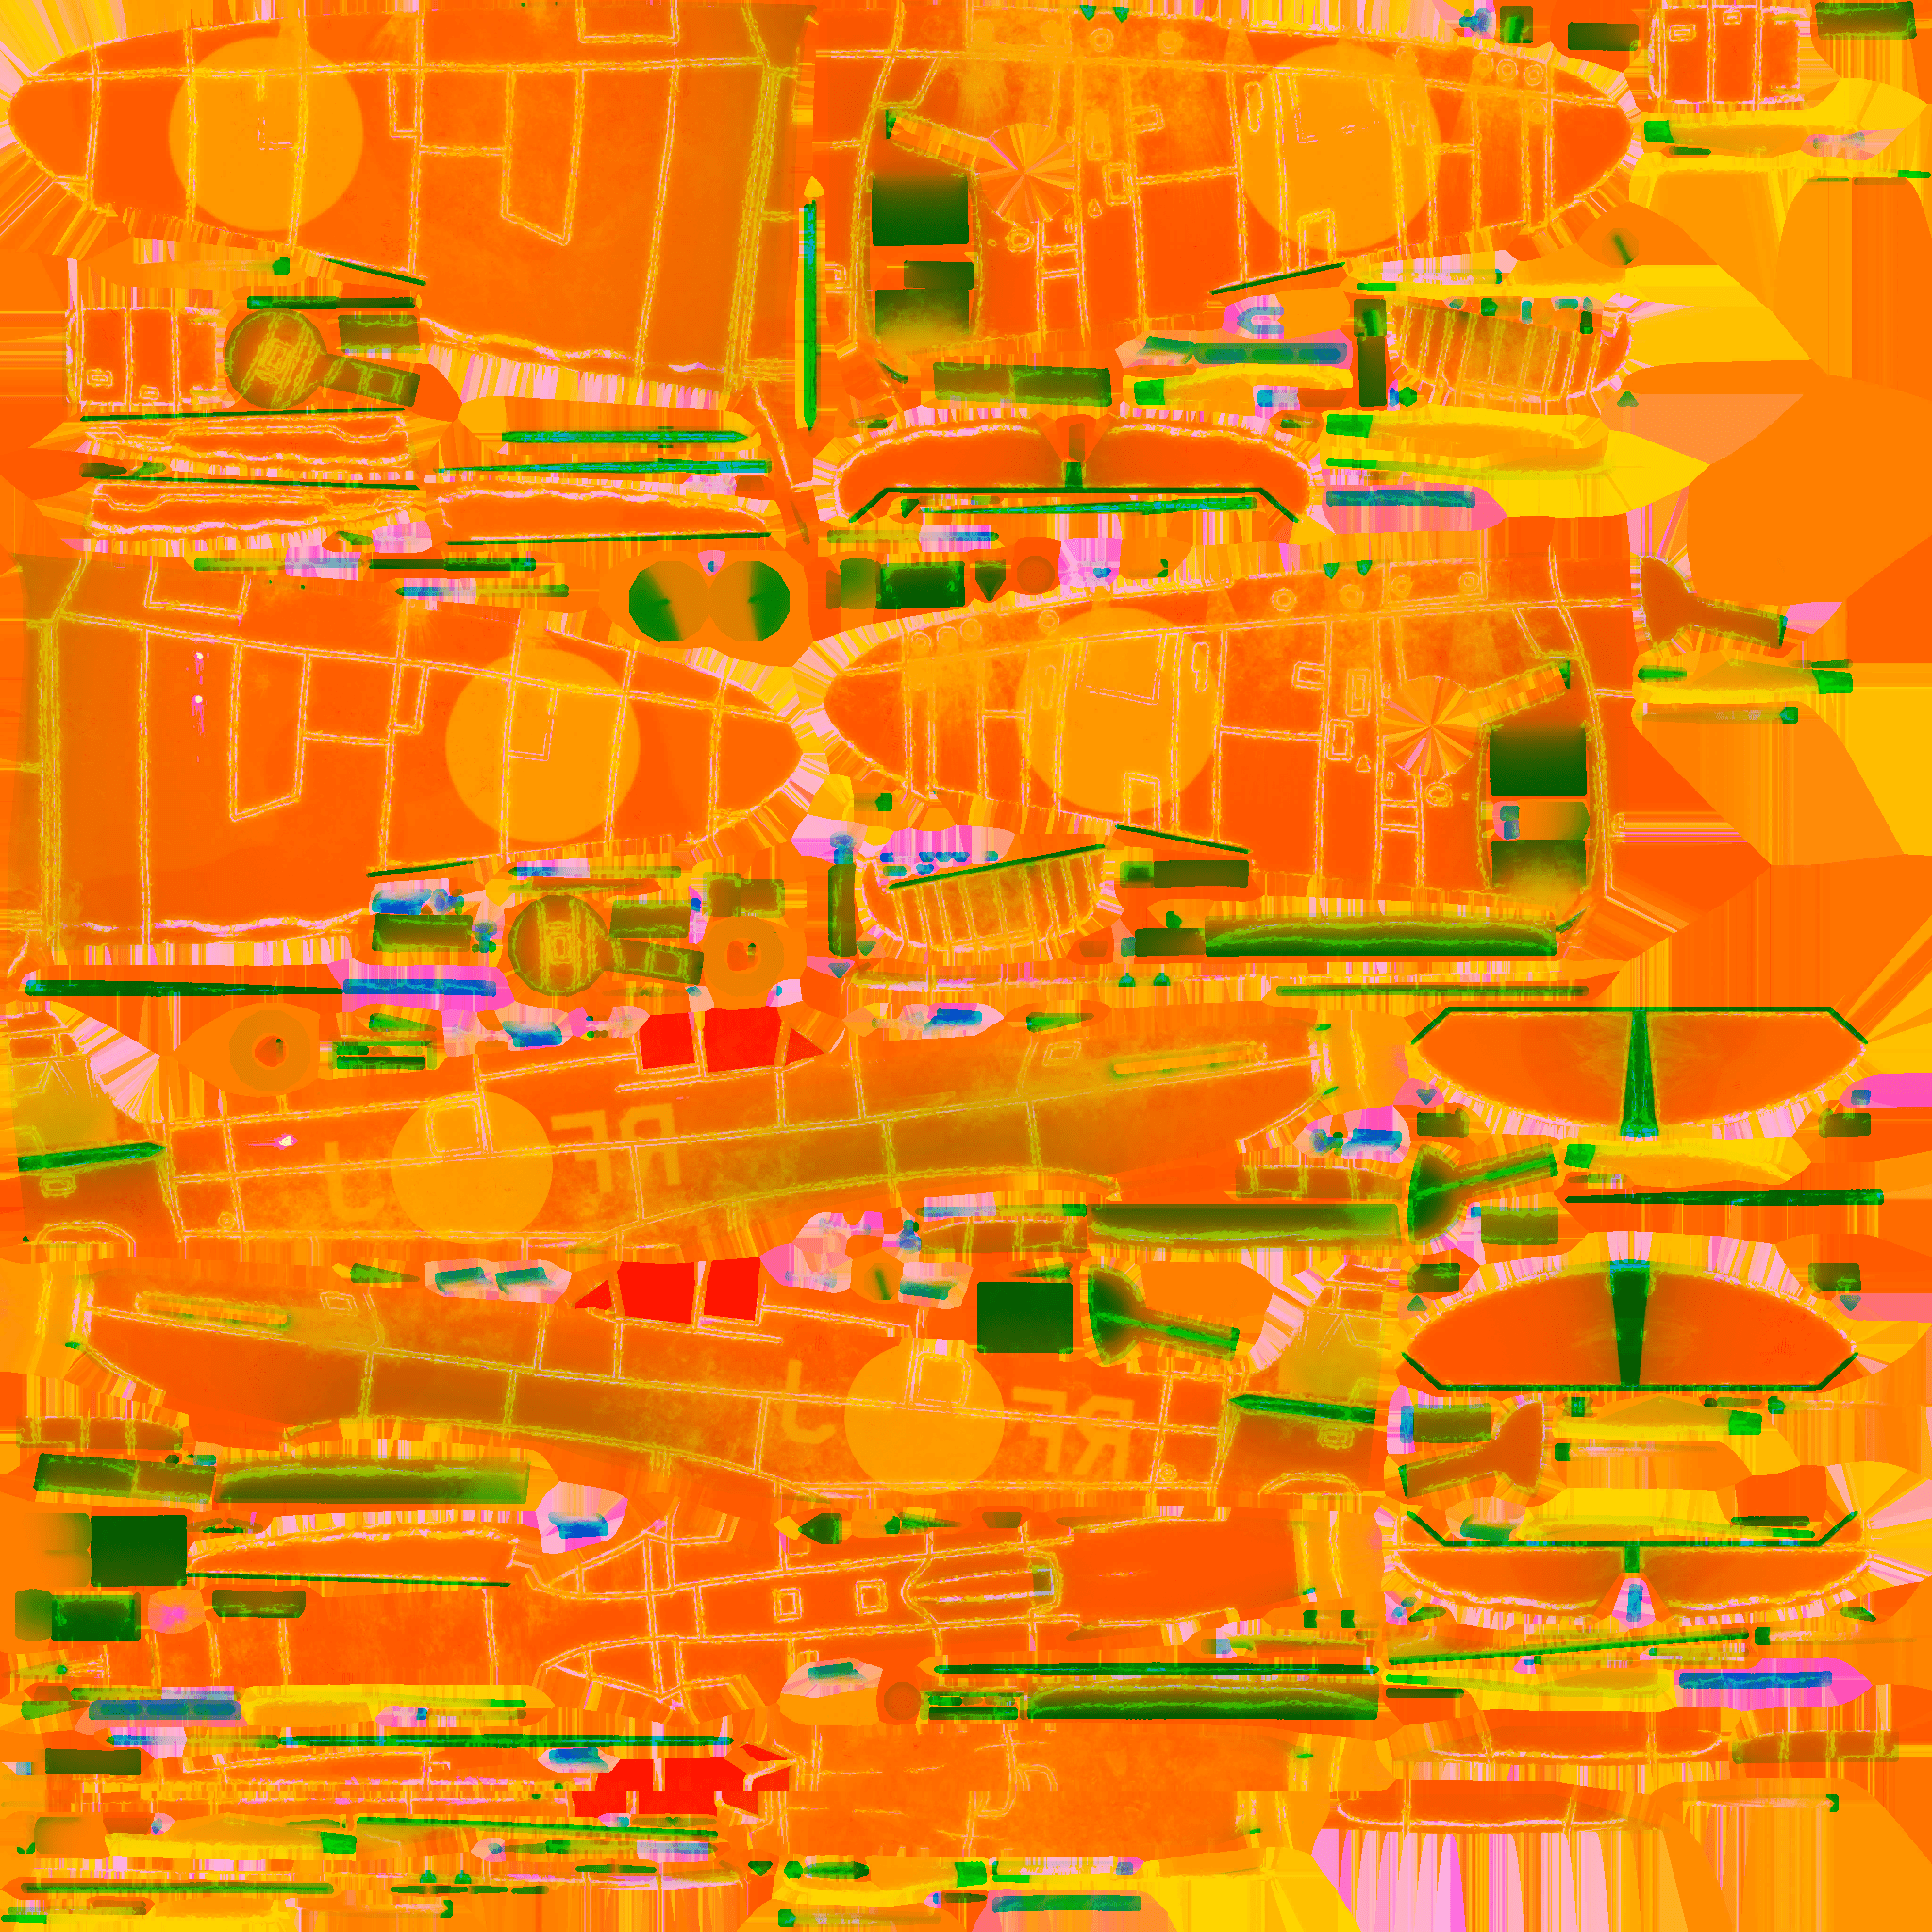
\includegraphics[width=0.4\textwidth]{pbrMaterial.png}}{\textcopyright kryik1023\\Sketchfab }
		& 
		\copyrightbox[r]{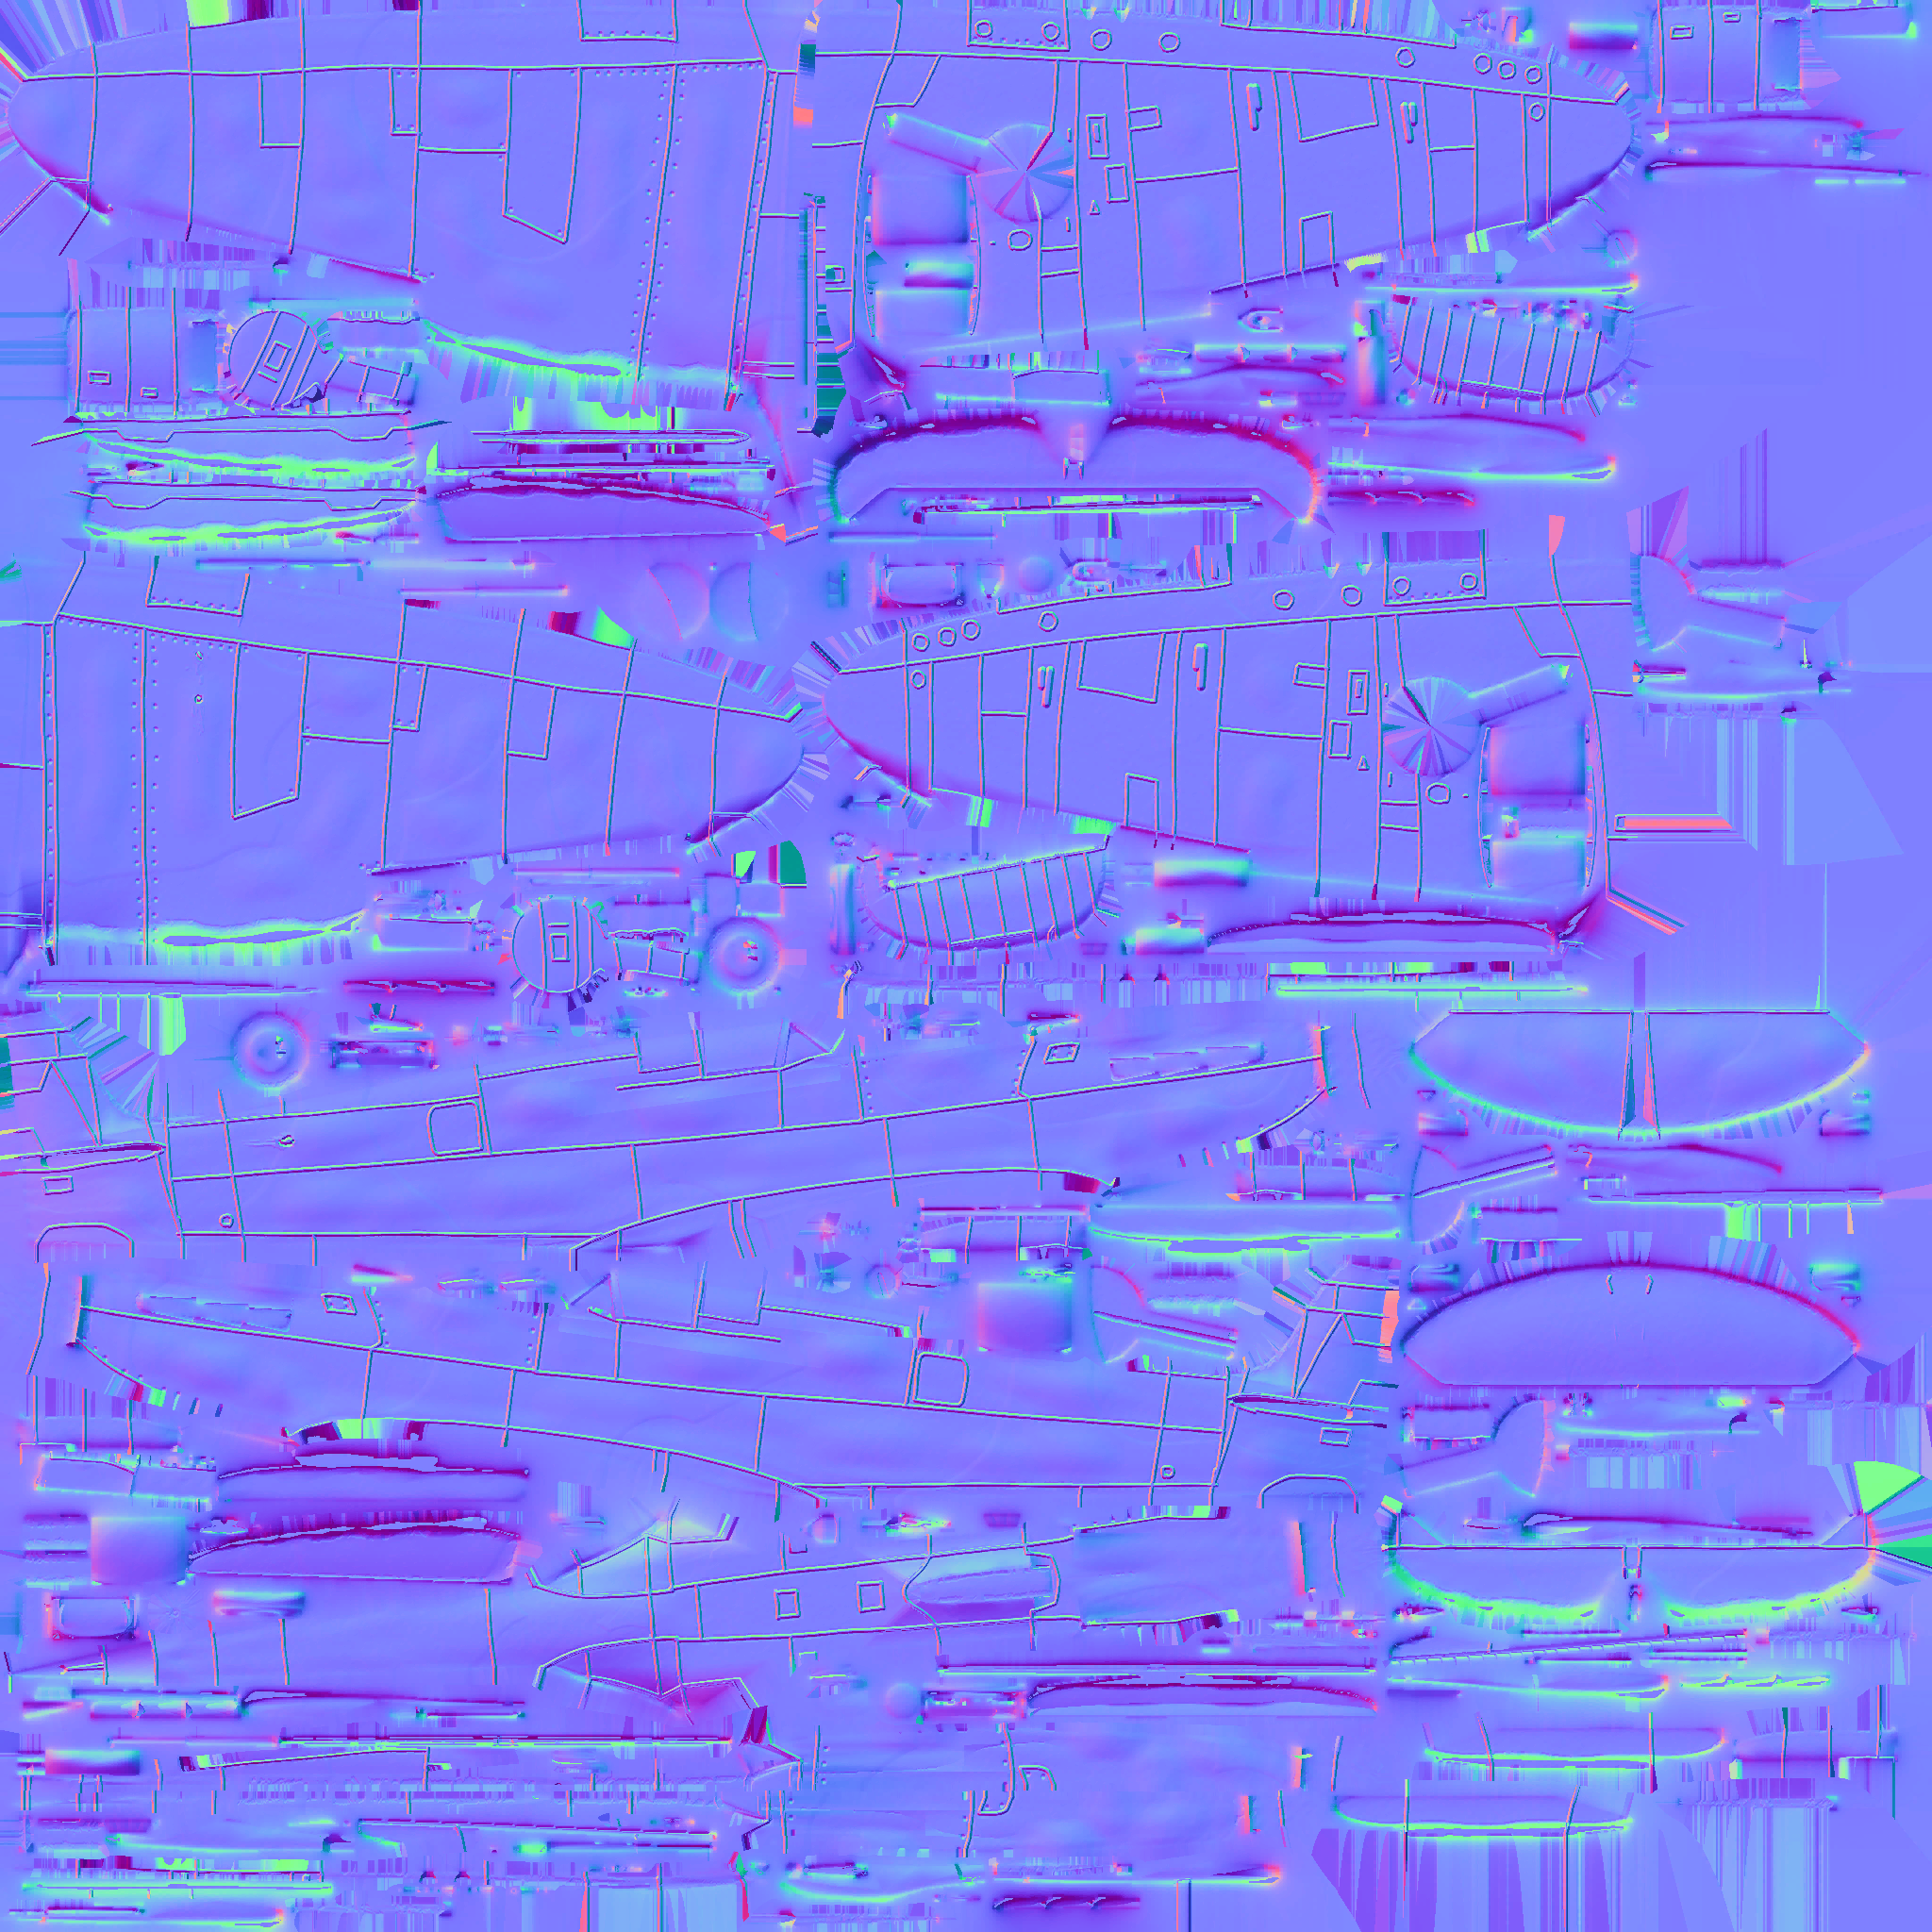
\includegraphics[width=0.4\textwidth]{pbrNormal.png}}{\textcopyright kryik1023\\Sketchfab }
		\\
		\caption{Przykładowy materiał wykorzystywany w PBR kodujący ambient occlusion w kanale czerwonym, chropowatość w zielonym, a metaliczność w niebieskim.}
		\label{pbrMaterial}
		&   \caption{Przykładowa mapa normalnych w przestrzeni stycznej.}
		\label{pbrNormal}
	\end{tabular}
\end{figure}

W przypadku naszej implementacji założono, że model będzie opierał się na modelu mikropowierzchni, zasady zachowania energii oraz wykorzystywał funkcję BRDF bazującą na fizyce.
\\

Model mikropowierzchni zakłada, że każda powierzchnia w mikroskopijnej skali może zostać opisana poprzez zestaw małych doskonałych zwierciadeł ustawionych pod różnymi kątami nazywanych mikropowierzchniami. Wtedy, gładkość powierzchni materiału może zostać opisana poprzez proporcję mikropowierzchni, które w przybliżeniu są ustawione zgodnie z pewnym wektorem $h$. Tym wektorem jest wektor połowicznej drogi (ang. halfway vector) między wektorem światła $l$ oraz wektorem obserwatora $v$, który wyznacza się zgodnie z równaniem \ref{halfway}.

\begin{equation}
	h= \frac{l + v}{\|l + \||}.
	\label{halfway}
\end{equation}

\color{red}`
Zasada zachowania energii mówi nam ponadto, że dla materiałów nie emitujących własnego światła, energia odbita od powierzchni nie może przewyższyć energii pobranej z otoczenia. Na tej podstawie mając ilość światła odbitego można wyznaczyć część światła, która zostanie rozproszona w materiale.
\color{black}
\\


Efekty uzyskane dzięki metodzie PBR zwizualizowano na rysunkach (\ref{phongCom}) i (\ref{pbrCom}), gdzie porównano je z prostszym, powszechnie używanym modelem oświetlenia Blinna-Phonga.
\\

\begin{figure}[h]
	\centering
	\setkeys{Gin}{width=\textwidth}
	\begin{tabular}{p{0.45\textwidth}p{0.45\textwidth}}
		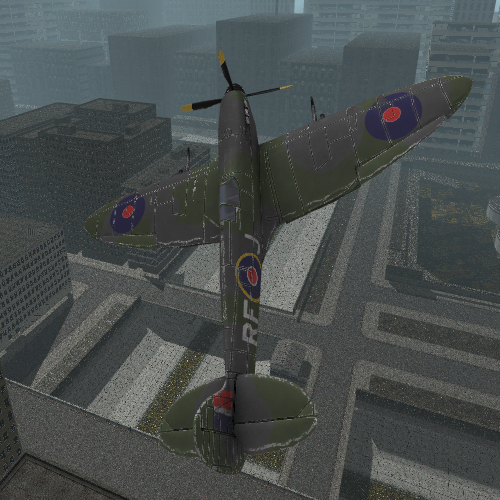
\includegraphics[width=0.45\textwidth]{phongComparison.png}
		& 
		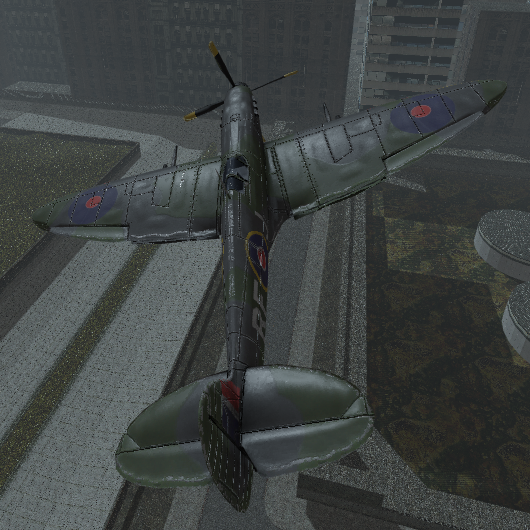
\includegraphics[width=0.45\textwidth]{pbrComparison.png}
		\\
		\caption{Model oświetlony z wykorzystaniem modelu Blinna-Phonga.}
		\label{phongCom}
		&   \caption{Model oświetlony z wykorzystaniem podejścia PBR.}
		\label{pbrCom}
	\end{tabular}
\end{figure}

Jednym z problemów podejścia PBR jest wymóg zapewnienia dodatkowych tekstur określających parametry fizyczne. Ich brak może doprowadzić do dysonansu między modelami bardziej i mniej dopracowanymi.
\\


\subsubsection{Cienie}

\color{red}
Coś tam coś tam o cieniach i procesie renderowania cieni.
\color{black}


\begin{figure}[h]
	\centering
	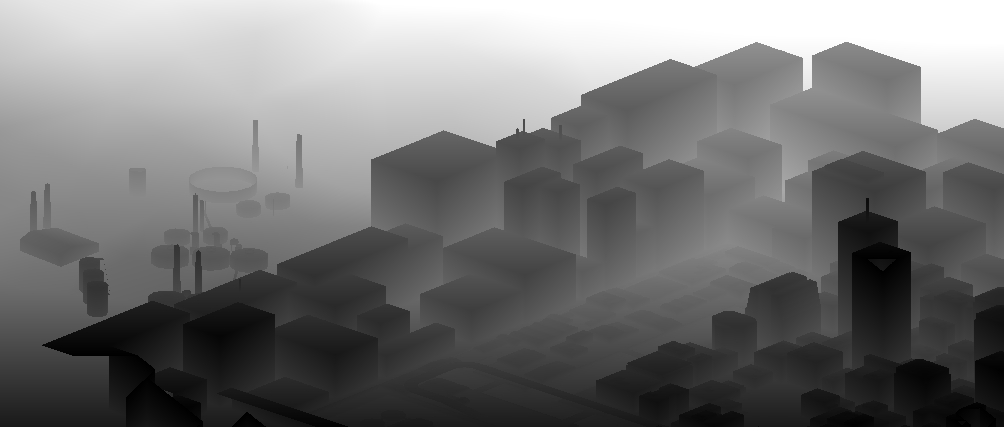
\includegraphics[width=0.9\textwidth]{shadowMap.png}
	\caption{Mapa głębi wykorzystywana przy sprawdzaniu czy przetwarzany fragment znajduje się w cieniu.}
	\label{shadowMap}
\end{figure}


\begin{figure}[h]
	\centering
	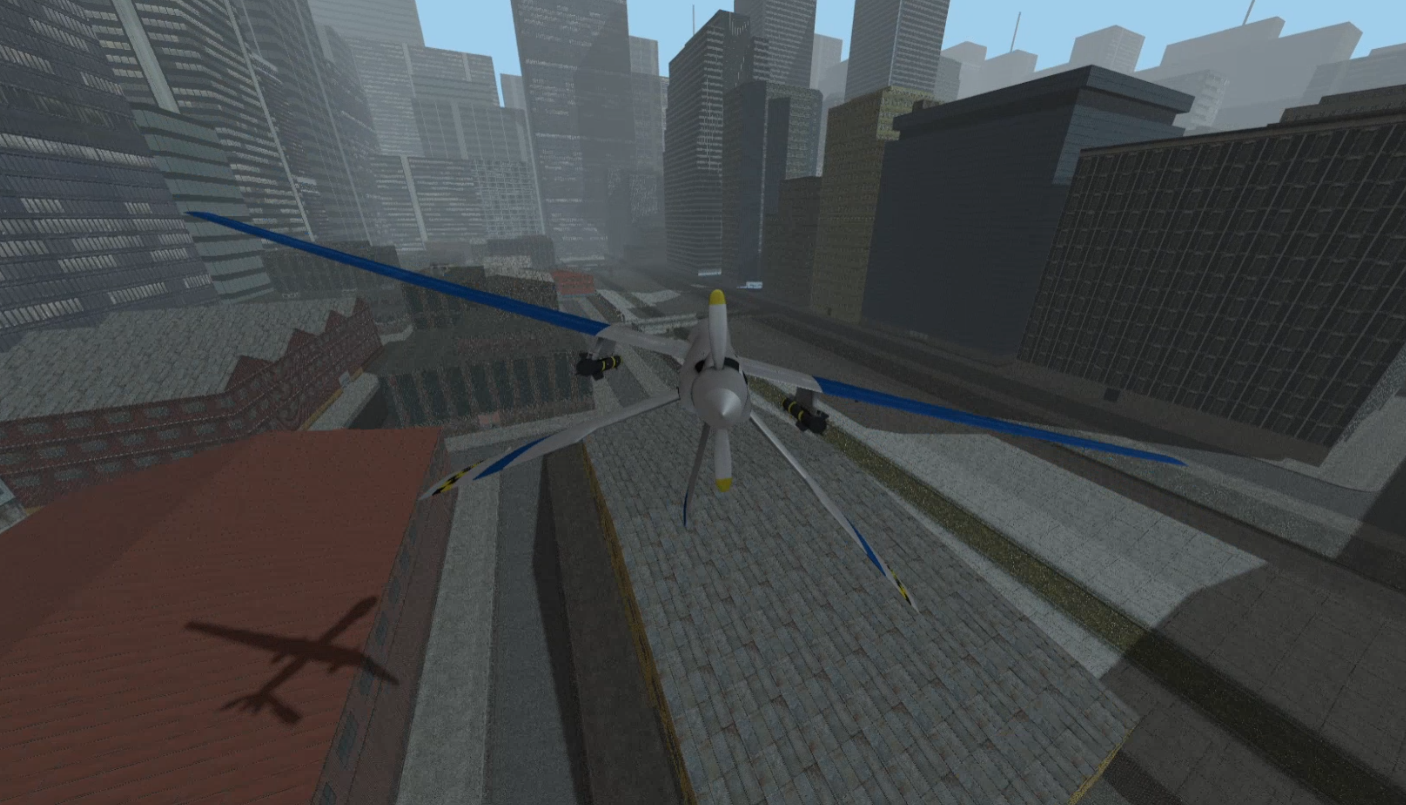
\includegraphics[width=0.9\textwidth]{shadows.png}
	\caption{Cień BSP oraz cienie budynków w oddali.}
	\label{shadows}
\end{figure}


\subsubsection{Rysowanie obwódki modelu za ścianą}

Jednym z początkowych problemów wizualizacji był brak widoczności modelu gdy między nim, a kamerą znajdywała się przeszkoda. Zdecydowano się na rozwiązanie tego problemu za pomocą zielonej obwódki wokół modelu jak widać na rysunku \ref{outline}. 


\begin{figure}[h]
	\centering
	\setkeys{Gin}{width=\textwidth}
	x\begin{tabular}{p{0.45\textwidth}p{0.45\textwidth}}
		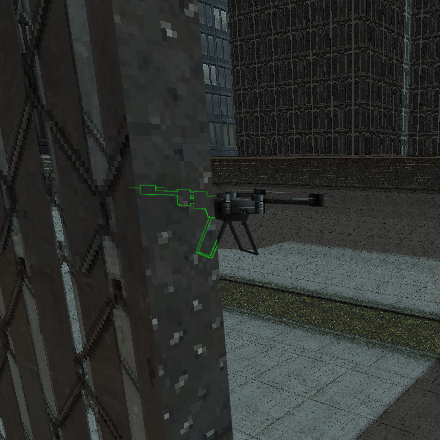
\includegraphics[width=0.45\textwidth]{outline.png}
		& 
		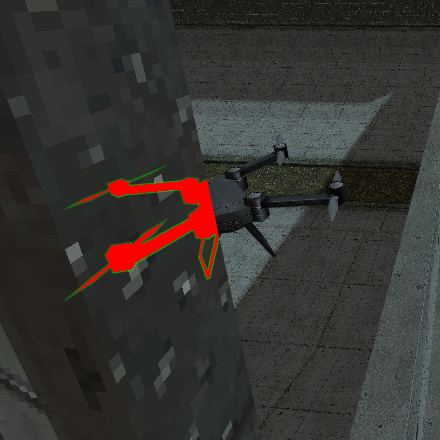
\includegraphics[width=0.45\textwidth]{outlineDebug.png}
		\\
		\caption{Zielona obwódka jest widoczna, gdy między BSP użytkownika a kamerą znajduje się przeszkoda.}
		\label{outline}
		&   
		\caption{Zielona obwódka wraz z maską wykorzystywaną do jej obliczenia.}
		\label{outlineDebug}
	\end{tabular}
\end{figure}

\color{red}
Stencil test. Moving with camera bo bufor jest ograniczony przez wartości.
Chanigng depth func etc.
\color{black}

\subsubsection{Ślad po wystrzelonym pocisku}

Przy implementacji pocisków zauważono, że małe pociski przy odpowiednio wysokiej prędkości są praktycznie niezauważalne. Dotyczy to na przykład nabojów broni palnej. Sam model pojawia się na ekranie wyłącznie przez kilka klatek. Aby zaradzić temu zdecydowano się na dodanie pociskom śladu. Jest to oddzielny shader operujący bez bufora wierzchołkowego, a więc wyłącznie z wykorzystaniem bufora uniform. Shader jest uruchamiany dla każdego pocisku i wykorzystuje $n$ zapisanych ostatnich jego pozycji. Na podstawie tych pozycji shader geometrii tworzy line strip rozpoczynający się od obecnej pozycji pocisku i kończący na ostatnim zapisanym punkcie zwiększając w każdym węźle przezroczystość linii. Dzięki zastosowaniu śladu pocisku, użytkownik jest w stanie lepiej zorientować się w jakim kierunku pocisk poleciał, a nawet zauważyć potencjalne rykoszety związane z mechanizmem wykrywania kolizji.

\subsubsection{Rysowanie liny}



\subsubsection{Wyznaczenie parametrów panelu śmigieł}

Panel śmigieł, rys. (\ref{smigla}), jest częścią graficznego interfejsu użytkownika i widoczny jest w prawym dolnym rogu ekranu. Informuje użytkownika o liczbie obrotów na minutę poszczególnych silników statku wraz z kierunkiem ich obrotu. Położenie śmigieł na panelu jest generowane proceduralnie na podstawie konfiguracji BSP podczas inicjalizacji aplikacji. Algorytm bierze pod uwagę konfigurację panelu w postaci marginesu oraz paddingu poszczególnych śmigieł oraz wysokość i minimalną szerokość okna tekstu. Zwraca uwagę również na odległości względne śmigieł w konfiguracji statku oraz kierunek, w którym się obracają. Na rysunku (\ref{smiglaDebug}) został zaprezentowany podgląd deweloperski panelu, który koloruje poszczególne jego części, a na rysunku (\ref{smiglaDebugRandom}) pokazane są możliwości algorytmu dla losowego rozmieszczenia śmigieł na BSP.
\\

Początkowo próbowano znaleźć parametry panelu za pomocą równań matematycznych. Z powodu skomplikowanych zależności zdecydowano się na podejście iteracyjne, które byłoby uruchamiane raz podczas inicjalizacji aplikacji. Zaprojektowany algorytm wykorzystuje podejście dziel i zwyciężaj szukając rozwiązanie w pikselach na przedziale $[1,\text{canvasSize}/2]$. Program bierze środkowy element obecnie analizowanego przedziału i sprawdza czy wybrany promień się mieści w ustalonych ograniczeniach. Jeżeli się udaje, to próbuje promień większy w podprzedziale z prawej strony elementu, w przeciwnym wypadku rozmiar mniejszy w podprzedziale z lewej strony.


\begin{figure}[h]
	\centering
	\setkeys{Gin}{width=\textwidth}
	\begin{tabular}{p{0.45\textwidth}p{0.45\textwidth}}
		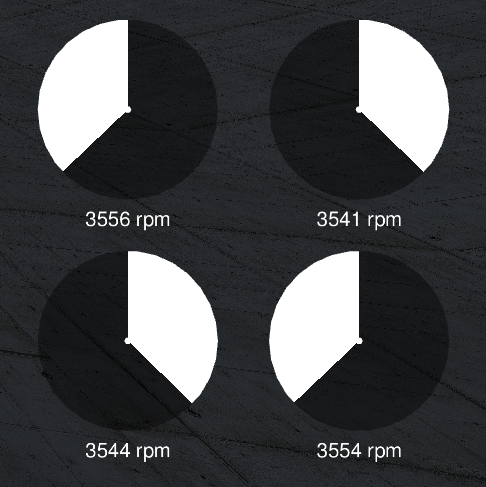
\includegraphics[width=0.45\textwidth]{smigla.png}
		& 
		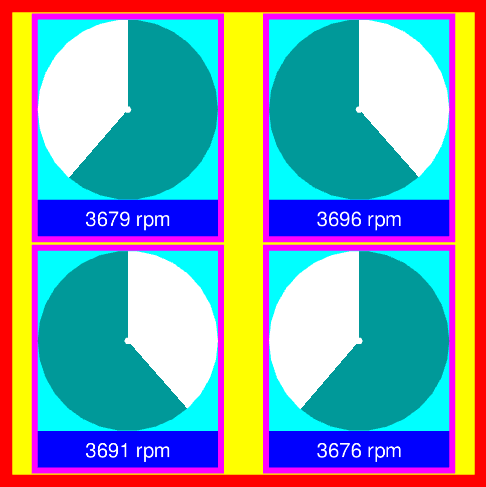
\includegraphics[width=0.45\textwidth]{smiglaDebug.png}
		\\
		\caption{Panel śmigieł jak widoczny w wizualizacji.}
		\label{smigla}
		&   \caption{Panel śmigieł w trybie deweloperskim pokazujący margines, padding oraz miejsce przeznaczone na poszczególne śmigła oraz tekst.}
		\label{smiglaDebug}
	\end{tabular}
\end{figure}

\begin{figure}[h]
	\centering
	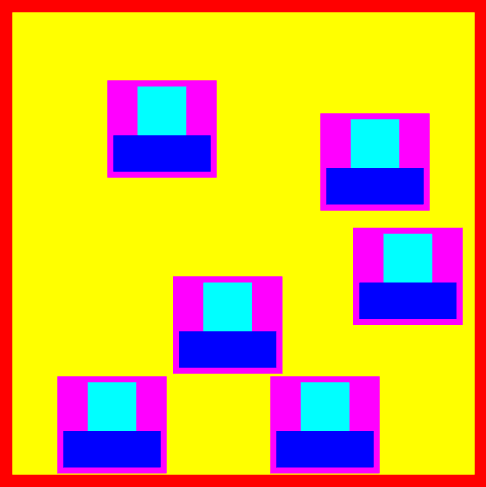
\includegraphics[width=0.5\textwidth]{smiglaDebugRandom.png}
	\caption{Pokazanie możliwości algorytmu generowania panelu śmigieł dla ich losowego rozmieszczenia. Są zachowane odległości i uwzględniona  jest minimalna szerokość panelu tekstu.}
	\label{smiglaDebugRandom}
\end{figure}


\subsubsection{Rysowanie radaru}
\subsubsection{Udźwiękowienie}

Udźwiękowienie symulatora zostało zrealizowane za pomocą implementacji standardu OpenAL. Dzieli się ono na muzykę oraz dźwięk śmigieł. Muzyka, która jest odtwarzana w tle, jest pobierana z katalogu wyznaczonego przez użytkownika losowo wybierając utwory w momencie gdy poprzedni się zakończy. Użytkownik również odpowiada za uzupełnienie folderu plikami o formacie OGG, które będą odtwarzane. Dźwięk śmigieł natomiast jest częścią symulacji i wykorzystuje bardziej zaawansowane funkcjonalności OpenAL. 
\\

Każdy dźwięk w OpenAL może być reprezentowany przez jego położenie, prędkość, głośność oraz wysokość. W ten sposób każde śmigło może wygenerować swój własny dźwięk. Ma on swoje położenie wyznaczane z wykorzystaniem parametru przesunięcia śmigła względem środka BSP i pozycji samego BSP we świecie oraz prędkość, która dla uproszczenia jest prędkością statku. Uznano, że głośność oraz wysokość dźwięku śmigła jest proporcjonalna do liczby obrotów na sekundę, gdzie dźwięk jest tym głośniejszy i wyższy, im szybciej śmigło się obraca. Z racji, że głośności różnych źródeł dźwięku się sumują, zdecydowano się, w celu zwiększenia komfortu pracy, na znormalizowanie głośności poprzez podzielenie jej przez liczbę rotorów BSP. 
\\

W OpenAL istnieje również koncept słuchacza, który tak samo jak źródło ma swoją pozycję oraz prędkość. Jest ona zawsze ustawiana na obecne położenie oraz prędkość kamery. Dzięki temu głośność dźwięku słyszanego przez użytkownika jest odwrotnie proporcjonalna do odległości kamery od źródła oraz zaobserwować można efekt stereo w kamerze pierwszoosobowej jak i efekt Dopplera.
\\

\subsubsection{Obsługa kontrolerów}

\subsubsection{Animacja modelu}


\color{red}
Jak się ogólnie ogarnia animacje w formacie glTF. Animacja w zależności od nazwy mesha i warunków zewnętrznych. Dać przykład śmigła i obrotów na sekundę oraz odchylenia powierzchni sterowych i joysticka oraz zrzucanie bomb jako skala 0. Jak animacje są ustandaryzowane.
\color{black}